\PassOptionsToPackage{unicode=true}{hyperref} % options for packages loaded elsewhere
\PassOptionsToPackage{hyphens}{url}
%
\documentclass[]{article}
\usepackage{lmodern}
\usepackage{amssymb,amsmath}
\usepackage{ifxetex,ifluatex}
\usepackage{fixltx2e} % provides \textsubscript
\ifnum 0\ifxetex 1\fi\ifluatex 1\fi=0 % if pdftex
  \usepackage[T1]{fontenc}
  \usepackage[utf8]{inputenc}
  \usepackage{textcomp} % provides euro and other symbols
\else % if luatex or xelatex
  \usepackage{unicode-math}
  \defaultfontfeatures{Ligatures=TeX,Scale=MatchLowercase}
\fi
% use upquote if available, for straight quotes in verbatim environments
\IfFileExists{upquote.sty}{\usepackage{upquote}}{}
% use microtype if available
\IfFileExists{microtype.sty}{%
\usepackage[]{microtype}
\UseMicrotypeSet[protrusion]{basicmath} % disable protrusion for tt fonts
}{}
\IfFileExists{parskip.sty}{%
\usepackage{parskip}
}{% else
\setlength{\parindent}{0pt}
\setlength{\parskip}{6pt plus 2pt minus 1pt}
}
\usepackage{hyperref}
\hypersetup{
            pdftitle={Topic 1: Exercise 1},
            pdfauthor={Daniel Alonso},
            pdfborder={0 0 0},
            breaklinks=true}
\urlstyle{same}  % don't use monospace font for urls
\usepackage[margin=1in]{geometry}
\usepackage{color}
\usepackage{fancyvrb}
\newcommand{\VerbBar}{|}
\newcommand{\VERB}{\Verb[commandchars=\\\{\}]}
\DefineVerbatimEnvironment{Highlighting}{Verbatim}{commandchars=\\\{\}}
% Add ',fontsize=\small' for more characters per line
\usepackage{framed}
\definecolor{shadecolor}{RGB}{248,248,248}
\newenvironment{Shaded}{\begin{snugshade}}{\end{snugshade}}
\newcommand{\AlertTok}[1]{\textcolor[rgb]{0.94,0.16,0.16}{#1}}
\newcommand{\AnnotationTok}[1]{\textcolor[rgb]{0.56,0.35,0.01}{\textbf{\textit{#1}}}}
\newcommand{\AttributeTok}[1]{\textcolor[rgb]{0.77,0.63,0.00}{#1}}
\newcommand{\BaseNTok}[1]{\textcolor[rgb]{0.00,0.00,0.81}{#1}}
\newcommand{\BuiltInTok}[1]{#1}
\newcommand{\CharTok}[1]{\textcolor[rgb]{0.31,0.60,0.02}{#1}}
\newcommand{\CommentTok}[1]{\textcolor[rgb]{0.56,0.35,0.01}{\textit{#1}}}
\newcommand{\CommentVarTok}[1]{\textcolor[rgb]{0.56,0.35,0.01}{\textbf{\textit{#1}}}}
\newcommand{\ConstantTok}[1]{\textcolor[rgb]{0.00,0.00,0.00}{#1}}
\newcommand{\ControlFlowTok}[1]{\textcolor[rgb]{0.13,0.29,0.53}{\textbf{#1}}}
\newcommand{\DataTypeTok}[1]{\textcolor[rgb]{0.13,0.29,0.53}{#1}}
\newcommand{\DecValTok}[1]{\textcolor[rgb]{0.00,0.00,0.81}{#1}}
\newcommand{\DocumentationTok}[1]{\textcolor[rgb]{0.56,0.35,0.01}{\textbf{\textit{#1}}}}
\newcommand{\ErrorTok}[1]{\textcolor[rgb]{0.64,0.00,0.00}{\textbf{#1}}}
\newcommand{\ExtensionTok}[1]{#1}
\newcommand{\FloatTok}[1]{\textcolor[rgb]{0.00,0.00,0.81}{#1}}
\newcommand{\FunctionTok}[1]{\textcolor[rgb]{0.00,0.00,0.00}{#1}}
\newcommand{\ImportTok}[1]{#1}
\newcommand{\InformationTok}[1]{\textcolor[rgb]{0.56,0.35,0.01}{\textbf{\textit{#1}}}}
\newcommand{\KeywordTok}[1]{\textcolor[rgb]{0.13,0.29,0.53}{\textbf{#1}}}
\newcommand{\NormalTok}[1]{#1}
\newcommand{\OperatorTok}[1]{\textcolor[rgb]{0.81,0.36,0.00}{\textbf{#1}}}
\newcommand{\OtherTok}[1]{\textcolor[rgb]{0.56,0.35,0.01}{#1}}
\newcommand{\PreprocessorTok}[1]{\textcolor[rgb]{0.56,0.35,0.01}{\textit{#1}}}
\newcommand{\RegionMarkerTok}[1]{#1}
\newcommand{\SpecialCharTok}[1]{\textcolor[rgb]{0.00,0.00,0.00}{#1}}
\newcommand{\SpecialStringTok}[1]{\textcolor[rgb]{0.31,0.60,0.02}{#1}}
\newcommand{\StringTok}[1]{\textcolor[rgb]{0.31,0.60,0.02}{#1}}
\newcommand{\VariableTok}[1]{\textcolor[rgb]{0.00,0.00,0.00}{#1}}
\newcommand{\VerbatimStringTok}[1]{\textcolor[rgb]{0.31,0.60,0.02}{#1}}
\newcommand{\WarningTok}[1]{\textcolor[rgb]{0.56,0.35,0.01}{\textbf{\textit{#1}}}}
\usepackage{graphicx,grffile}
\makeatletter
\def\maxwidth{\ifdim\Gin@nat@width>\linewidth\linewidth\else\Gin@nat@width\fi}
\def\maxheight{\ifdim\Gin@nat@height>\textheight\textheight\else\Gin@nat@height\fi}
\makeatother
% Scale images if necessary, so that they will not overflow the page
% margins by default, and it is still possible to overwrite the defaults
% using explicit options in \includegraphics[width, height, ...]{}
\setkeys{Gin}{width=\maxwidth,height=\maxheight,keepaspectratio}
\setlength{\emergencystretch}{3em}  % prevent overfull lines
\providecommand{\tightlist}{%
  \setlength{\itemsep}{0pt}\setlength{\parskip}{0pt}}
\setcounter{secnumdepth}{0}
% Redefines (sub)paragraphs to behave more like sections
\ifx\paragraph\undefined\else
\let\oldparagraph\paragraph
\renewcommand{\paragraph}[1]{\oldparagraph{#1}\mbox{}}
\fi
\ifx\subparagraph\undefined\else
\let\oldsubparagraph\subparagraph
\renewcommand{\subparagraph}[1]{\oldsubparagraph{#1}\mbox{}}
\fi

% set default figure placement to htbp
\makeatletter
\def\fps@figure{htbp}
\makeatother


\title{Topic 1: Exercise 1}
\author{Daniel Alonso}
\date{November 15th, 2020}

\begin{document}
\maketitle

\hypertarget{importing-the-data}{%
\paragraph{Importing the data}\label{importing-the-data}}

\begin{Shaded}
\begin{Highlighting}[]
\KeywordTok{library}\NormalTok{(dplyr)}
\KeywordTok{library}\NormalTok{(stringr)}
\KeywordTok{library}\NormalTok{(PerformanceAnalytics)}
\KeywordTok{library}\NormalTok{(foreach)}
\KeywordTok{library}\NormalTok{(ggplot2)}
\KeywordTok{library}\NormalTok{(reshape2)}
\KeywordTok{library}\NormalTok{(MASS)}
\KeywordTok{library}\NormalTok{(andrews)}
\end{Highlighting}
\end{Shaded}

\begin{Shaded}
\begin{Highlighting}[]
\NormalTok{d <-}\StringTok{ }\KeywordTok{read.csv}\NormalTok{(}\StringTok{'../../datasets/Colleges.csv'}\NormalTok{)}
\end{Highlighting}
\end{Shaded}

\begin{Shaded}
\begin{Highlighting}[]
\KeywordTok{head}\NormalTok{(d)}
\end{Highlighting}
\end{Shaded}

\begin{verbatim}
##                                                X  Private Apps Accept Enroll
## 1 Abilene Christian University                   Yes      1660   1232    721
## 2 Adelphi University                             Yes      2186   1924    512
## 3 Adrian College                                 Yes      1428   1097    336
## 4 Agnes Scott College                            Yes       417    349    137
## 5 Alaska Pacific University                      Yes       193    146     55
## 6 Albertson College                              Yes       587    479    158
##   Top10perc Top25perc F.Undergrad P.Undergrad Outstate Room.Board Books
## 1        23        52        2885         537     7440       3300   450
## 2        16        29        2683        1227    12280       6450   750
## 3        22        50        1036          99    11250       3750   400
## 4        60        89         510          63    12960       5450   450
## 5        16        44         249         869     7560       4120   800
## 6        38        62         678          41    13500       3335   500
##   Personal PhD Terminal S.F.Ratio perc.alumni Expend Grad.Rate
## 1     2200  70       78      18.1          12   7041        60
## 2     1500  29       30      12.2          16  10527        56
## 3     1165  53       66      12.9          30   8735        54
## 4      875  92       97       7.7          37  19016        59
## 5     1500  76       72      11.9           2  10922        15
## 6      675  67       73       9.4          11   9727        55
\end{verbatim}

\hypertarget{identify-the-type-of-all-variables}{%
\subsection{1- Identify the type of all
variables}\label{identify-the-type-of-all-variables}}

\begin{Shaded}
\begin{Highlighting}[]
\KeywordTok{foreach}\NormalTok{ (}\DataTypeTok{col =}\NormalTok{ d, }\DataTypeTok{nms =} \KeywordTok{colnames}\NormalTok{(d)) }\OperatorTok\StringTok{ }\NormalTok{\{}
    \KeywordTok{print}\NormalTok{(}\KeywordTok{str_interp}\NormalTok{(}\StringTok{"$\{nms\} is of type $\{typeof(col)\}"}\NormalTok{))}
\NormalTok{\}}
\end{Highlighting}
\end{Shaded}

\hypertarget{represented-as-r-type---numericalcategorical}{%
\paragraph{represented as R type -
numerical/categorical}\label{represented-as-r-type---numericalcategorical}}

\begin{itemize}
\tightlist
\item
  X is of type character - categorical (id)
\item
  Private is of type character - categorical binary
\item
  Apps is of type integer - numerical discrete
\item
  Accept is of type integer - numerical discrete
\item
  Enroll is of type integer - numerical discrete
\item
  Top10perc is of type integer - numerical discrete
\item
  Top25perc is of type integer - numerical discrete
\item
  F.Undergrad is of type integer - numerical discrete
\item
  P.Undergrad is of type integer - numerical discrete
\item
  Outstate is of type integer - numerical discrete
\item
  Room.Board is of type integer - numerical discrete
\item
  Books is of type integer - numerical discrete
\item
  Personal is of type integer - numerical discrete
\item
  PhD is of type integer - numerical discrete
\item
  Terminal is of type integer - numerical discrete
\item
  S.F.Ratio is of type double - numerical continuous
\item
  perc.alumni is of type integer - numerical discrete
\item
  Expend is of type integer - numerical discrete
\item
  Grad.Rate is of type integer - numerical discrete
\end{itemize}

\hypertarget{perform-a-visual-analysis-of-each-quantitative-variable.-then-do-so-considering-the-variable-private.-describe-each-plot.}{%
\subsection{\texorpdfstring{2- Perform a visual analysis of each
quantitative variable. Then do so considering the variable
\emph{private}. Describe each
plot.}{2- Perform a visual analysis of each quantitative variable. Then do so considering the variable private. Describe each plot.}}\label{perform-a-visual-analysis-of-each-quantitative-variable.-then-do-so-considering-the-variable-private.-describe-each-plot.}}

\hypertarget{histograms}{%
\subsubsection{Histograms}\label{histograms}}

\begin{Shaded}
\begin{Highlighting}[]
\CommentTok{# setting plot sizes}
\KeywordTok{options}\NormalTok{(}\DataTypeTok{repr.plot.width =} \DecValTok{14}\NormalTok{, }\DataTypeTok{repr.plot.height =} \DecValTok{8}\NormalTok{)}
\end{Highlighting}
\end{Shaded}

\begin{Shaded}
\begin{Highlighting}[]
\CommentTok{# Apps}
\KeywordTok{hist}\NormalTok{(d}\OperatorTok{$}\NormalTok{Apps)}
\end{Highlighting}
\end{Shaded}

\includegraphics{Exercise_1_files/figure-latex/unnamed-chunk-6-1.pdf}

\begin{itemize}
\tightlist
\item
  Large right tail, higher frequency
\item
  Long left tail
\item
  Very right skewed
\item
  Resembles gamma distribution
\end{itemize}

\begin{Shaded}
\begin{Highlighting}[]
\CommentTok{# Accept}
\KeywordTok{hist}\NormalTok{(d}\OperatorTok{$}\NormalTok{Accept)}
\end{Highlighting}
\end{Shaded}

\includegraphics{Exercise_1_files/figure-latex/unnamed-chunk-7-1.pdf}

Pretty much the same as Apps but with a significantly shorter left tail.
Probably because those students being accepted are just a subset of
those that apply.

\begin{Shaded}
\begin{Highlighting}[]
\CommentTok{# Enroll}
\KeywordTok{hist}\NormalTok{(d}\OperatorTok{$}\NormalTok{Enroll)}
\end{Highlighting}
\end{Shaded}

\includegraphics{Exercise_1_files/figure-latex/unnamed-chunk-8-1.pdf}

Enroll also tells the same story, but in this case our left tail is even
smaller than the accept left tail. Maybe because significantly less
students enroll than those that just get accepted

\begin{Shaded}
\begin{Highlighting}[]
\CommentTok{# Top10perc}
\KeywordTok{hist}\NormalTok{(d}\OperatorTok{$}\NormalTok{Top10perc)}
\end{Highlighting}
\end{Shaded}

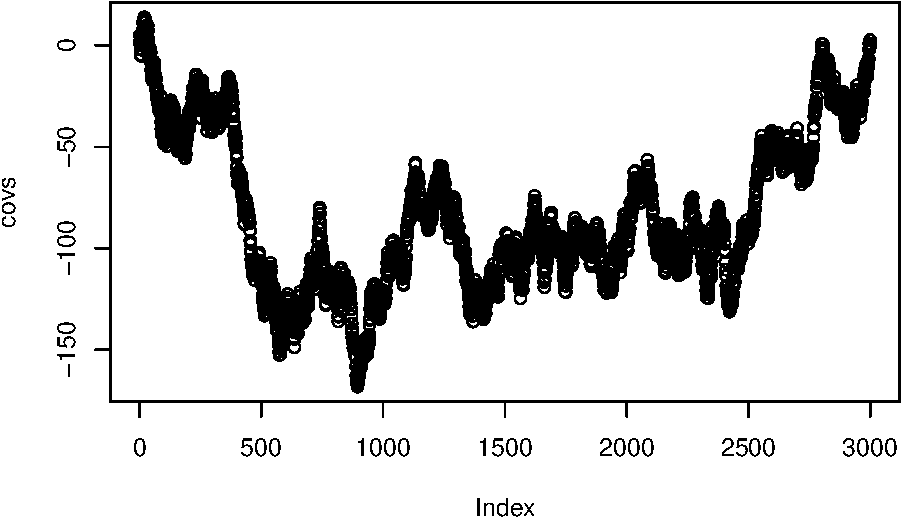
\includegraphics{Exercise_1_files/figure-latex/unnamed-chunk-9-1.pdf}

\begin{itemize}
\tightlist
\item
  long left tail
\item
  short but high frequency right tail
\item
  Resembles gaussian distribution
\item
  most elements concentrate around 20
\end{itemize}

\begin{Shaded}
\begin{Highlighting}[]
\CommentTok{# Top25perc}
\KeywordTok{hist}\NormalTok{(d}\OperatorTok{$}\NormalTok{Top25perc)}
\end{Highlighting}
\end{Shaded}

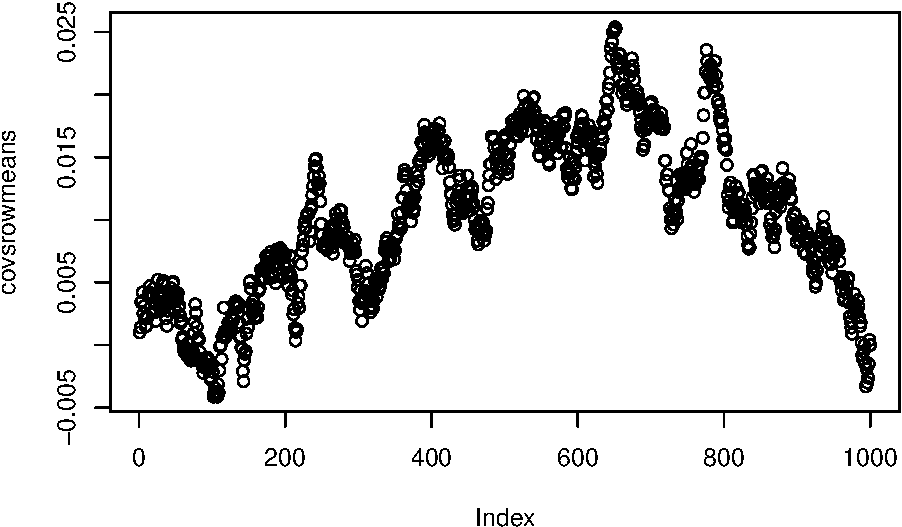
\includegraphics{Exercise_1_files/figure-latex/unnamed-chunk-10-1.pdf}

\begin{itemize}
\tightlist
\item
  mean is probably between 40-60
\item
  small right tail
\item
  large left tail
\item
  Resembles gaussian distribution
\end{itemize}

\begin{Shaded}
\begin{Highlighting}[]
\CommentTok{# F.Undergrad}
\KeywordTok{hist}\NormalTok{(d}\OperatorTok{$}\NormalTok{F.Undergrad)}
\end{Highlighting}
\end{Shaded}

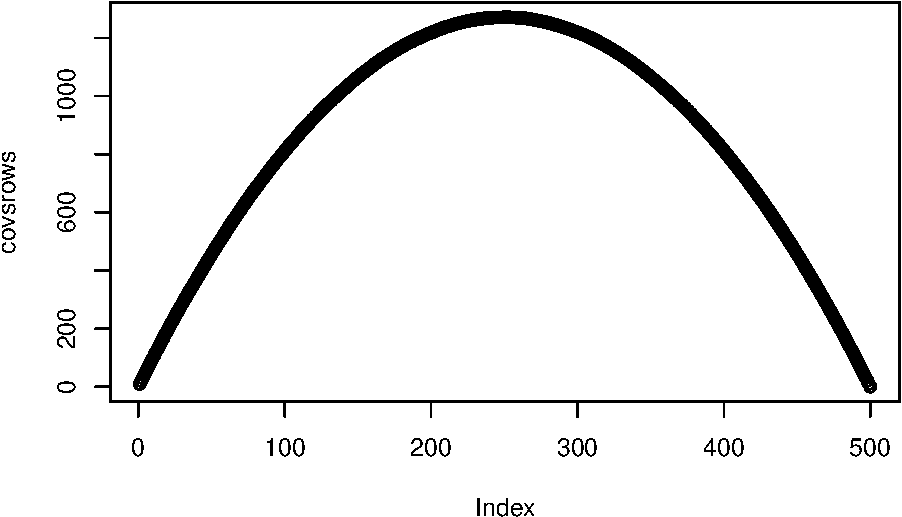
\includegraphics{Exercise_1_files/figure-latex/unnamed-chunk-11-1.pdf}

\begin{itemize}
\tightlist
\item
  long left tail
\item
  most of the universities between 0-5000
\item
  significantly less data at 5000+
\item
  Resembles gamma distribution
\end{itemize}

\begin{Shaded}
\begin{Highlighting}[]
\CommentTok{# P.Undergrad}
\KeywordTok{hist}\NormalTok{(d}\OperatorTok{$}\NormalTok{P.Undergrad)}
\end{Highlighting}
\end{Shaded}

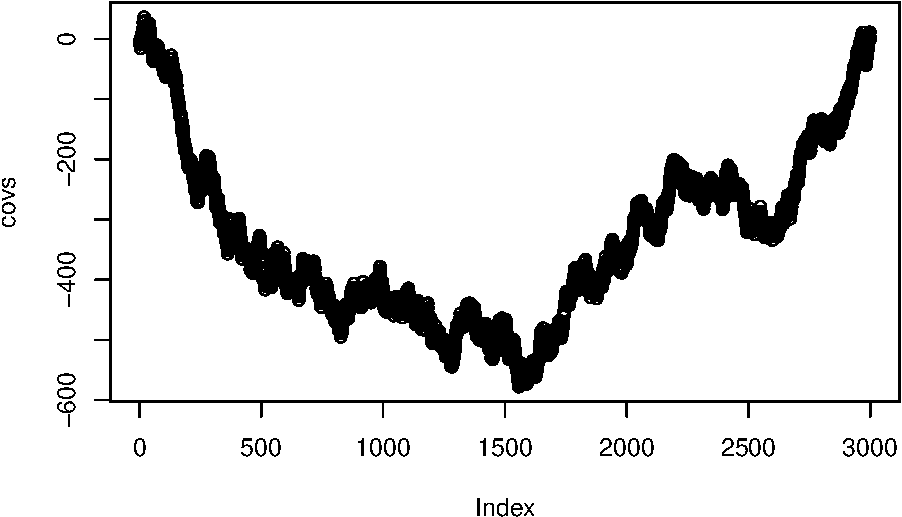
\includegraphics{Exercise_1_files/figure-latex/unnamed-chunk-12-1.pdf}

Similar to F.Undergrad we have a quite long right tail, this one
resembles Apps more, and similar to F.Undergrad we also have a large
frequency right tail and possibly more than 90\% of the data between 0
and 5000

\begin{Shaded}
\begin{Highlighting}[]
\CommentTok{# Outstate}
\KeywordTok{hist}\NormalTok{(d}\OperatorTok{$}\NormalTok{Outstate)}
\end{Highlighting}
\end{Shaded}

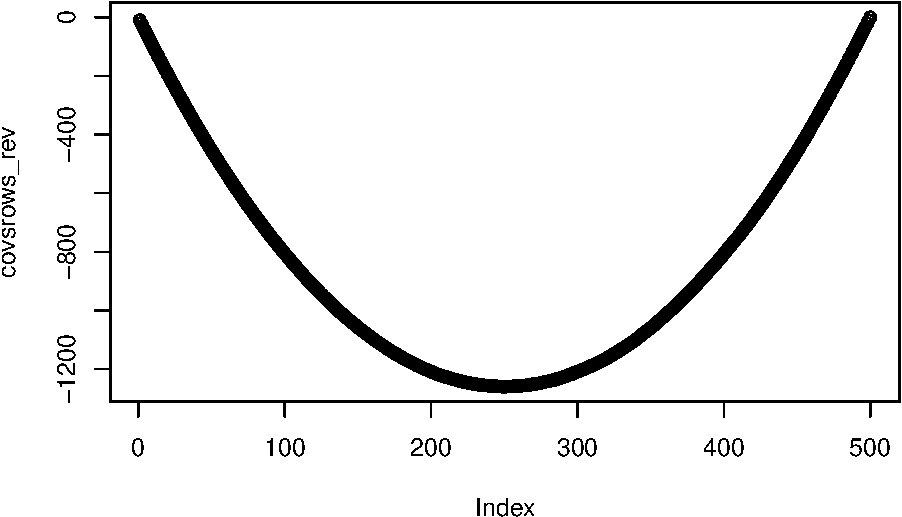
\includegraphics{Exercise_1_files/figure-latex/unnamed-chunk-13-1.pdf}

\begin{itemize}
\tightlist
\item
  Mean around 10000
\item
  relatively heavy left tail but not very long
\item
  light right tail
\item
  resembles gaussian distribution
\end{itemize}

\begin{Shaded}
\begin{Highlighting}[]
\CommentTok{# Room.Board}
\KeywordTok{hist}\NormalTok{(d}\OperatorTok{$}\NormalTok{Room.Board)}
\end{Highlighting}
\end{Shaded}

\includegraphics{Exercise_1_files/figure-latex/unnamed-chunk-14-1.pdf}

\begin{itemize}
\tightlist
\item
  resembles a slightly right skewed gaussian distribution
\item
  relatively long left tail
\item
  mean between 3500-4500
\end{itemize}

\begin{Shaded}
\begin{Highlighting}[]
\CommentTok{# Books}
\KeywordTok{hist}\NormalTok{(d}\OperatorTok{$}\NormalTok{Books)}
\end{Highlighting}
\end{Shaded}

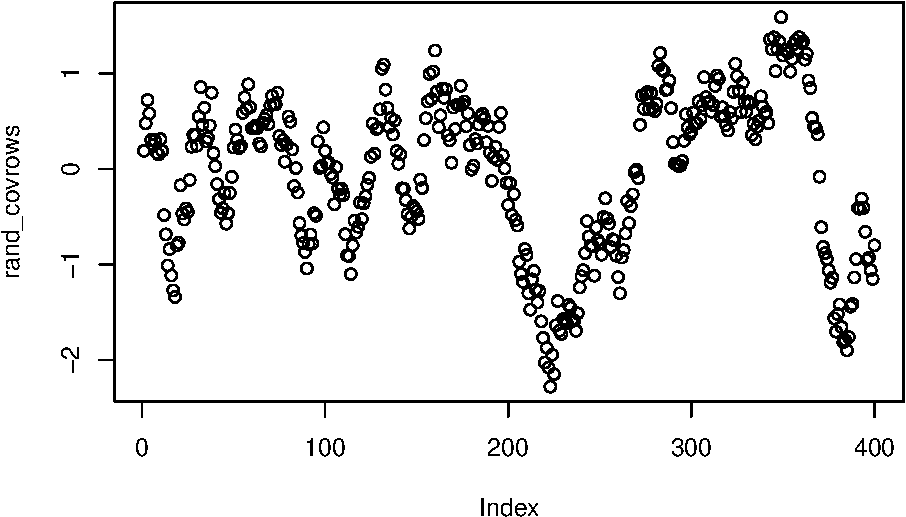
\includegraphics{Exercise_1_files/figure-latex/unnamed-chunk-15-1.pdf}

\begin{itemize}
\tightlist
\item
  long left tail
\item
  very right skewed
\item
  mean most probably around 500
\item
  nearly all values between 400-750
\end{itemize}

\begin{Shaded}
\begin{Highlighting}[]
\CommentTok{# Personal}
\KeywordTok{hist}\NormalTok{(d}\OperatorTok{$}\NormalTok{Personal)}
\end{Highlighting}
\end{Shaded}

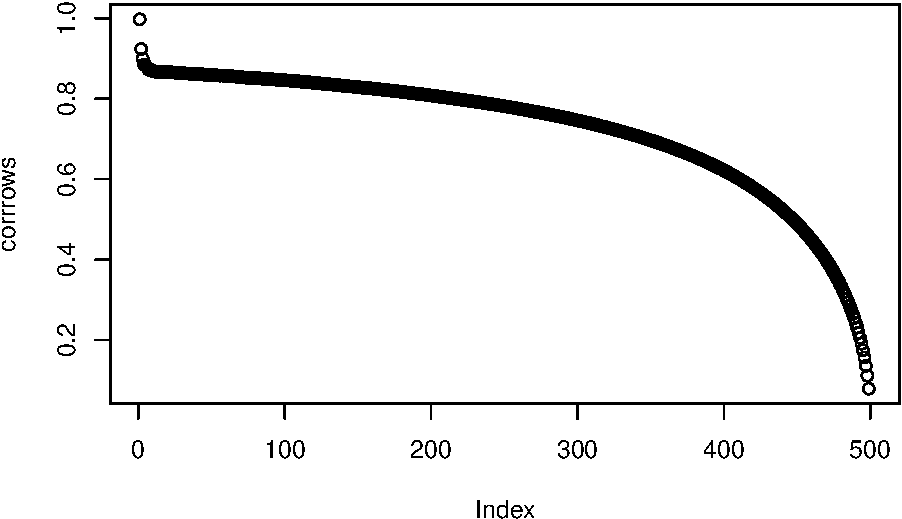
\includegraphics{Exercise_1_files/figure-latex/unnamed-chunk-16-1.pdf}

\begin{itemize}
\tightlist
\item
  very right skewed
\item
  long left tail
\item
  resembles a gamma distribution
\end{itemize}

\begin{Shaded}
\begin{Highlighting}[]
\CommentTok{# PhD}
\KeywordTok{hist}\NormalTok{(d}\OperatorTok{$}\NormalTok{PhD)}
\end{Highlighting}
\end{Shaded}

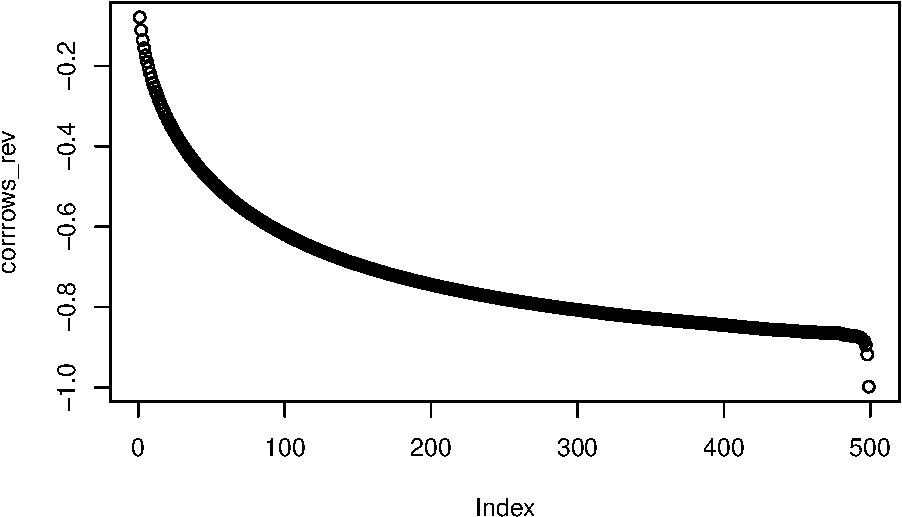
\includegraphics{Exercise_1_files/figure-latex/unnamed-chunk-17-1.pdf}

\begin{itemize}
\tightlist
\item
  long and light right tail
\item
  very left skewed
\end{itemize}

\begin{Shaded}
\begin{Highlighting}[]
\CommentTok{# Terminal}
\KeywordTok{hist}\NormalTok{(d}\OperatorTok{$}\NormalTok{Terminal)}
\end{Highlighting}
\end{Shaded}

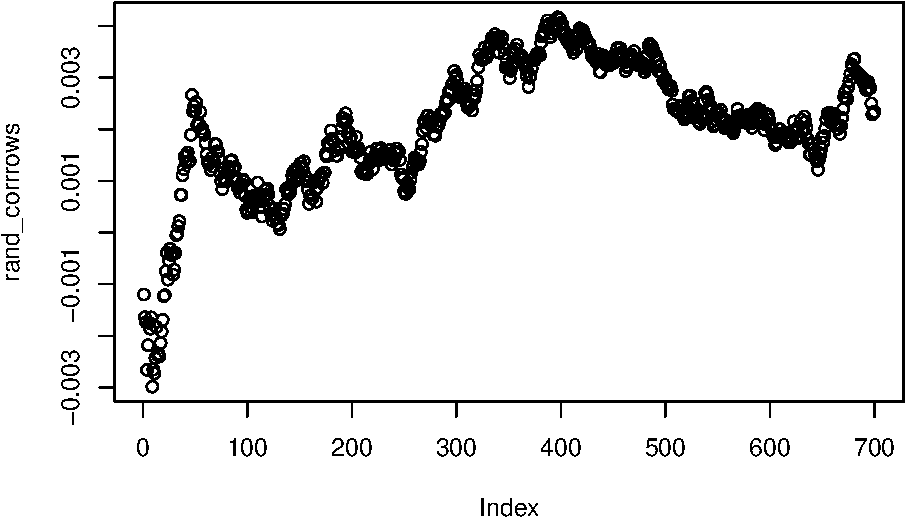
\includegraphics{Exercise_1_files/figure-latex/unnamed-chunk-18-1.pdf}

\begin{itemize}
\tightlist
\item
  very left skewed
\item
  light and long right tail
\item
  frequency increases with value (the higher the more common perhaps?)
\end{itemize}

\begin{Shaded}
\begin{Highlighting}[]
\CommentTok{# S.F.Ratio}
\KeywordTok{hist}\NormalTok{(d}\OperatorTok{$}\NormalTok{S.F.Ratio)}
\end{Highlighting}
\end{Shaded}

\includegraphics{Exercise_1_files/figure-latex/unnamed-chunk-19-1.pdf}

\begin{itemize}
\tightlist
\item
  most values between 10-20
\item
  light and long left tail
\item
  light right tail
\item
  resembles gaussian distribution
\end{itemize}

\begin{Shaded}
\begin{Highlighting}[]
\CommentTok{# perc.alumni}
\KeywordTok{hist}\NormalTok{(d}\OperatorTok{$}\NormalTok{perc.alumni)}
\end{Highlighting}
\end{Shaded}

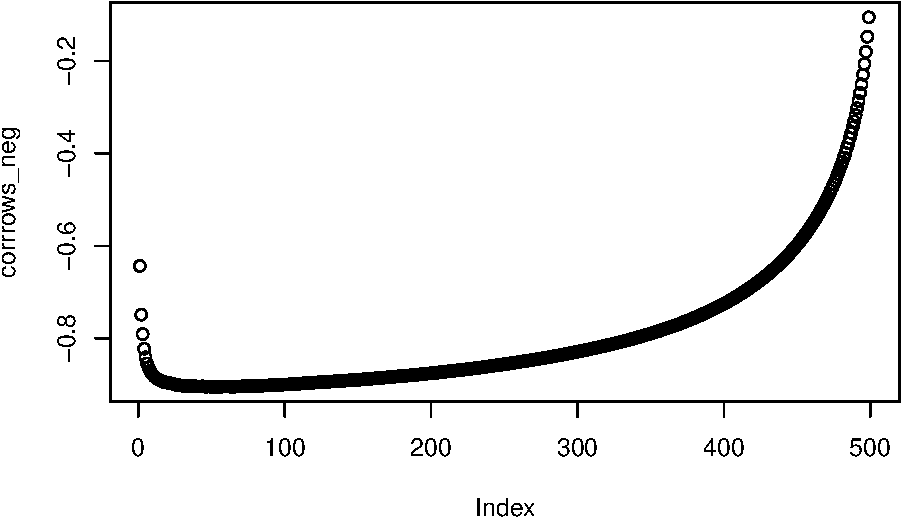
\includegraphics{Exercise_1_files/figure-latex/unnamed-chunk-20-1.pdf}

\begin{itemize}
\tightlist
\item
  right skewed
\item
  long and light left tail
\item
  relatively flat around the highest frequency part
\end{itemize}

\begin{Shaded}
\begin{Highlighting}[]
\CommentTok{# Expend}
\KeywordTok{hist}\NormalTok{(d}\OperatorTok{$}\NormalTok{Expend)}
\end{Highlighting}
\end{Shaded}

\includegraphics{Exercise_1_files/figure-latex/unnamed-chunk-21-1.pdf}

\begin{itemize}
\tightlist
\item
  very right skewed
\item
  very long left tail
\item
  most values around 10000
\item
  resembles gamma distribution
\end{itemize}

\begin{Shaded}
\begin{Highlighting}[]
\CommentTok{# Grad.Rate}
\KeywordTok{hist}\NormalTok{(d}\OperatorTok{$}\NormalTok{Grad.Rate)}
\end{Highlighting}
\end{Shaded}

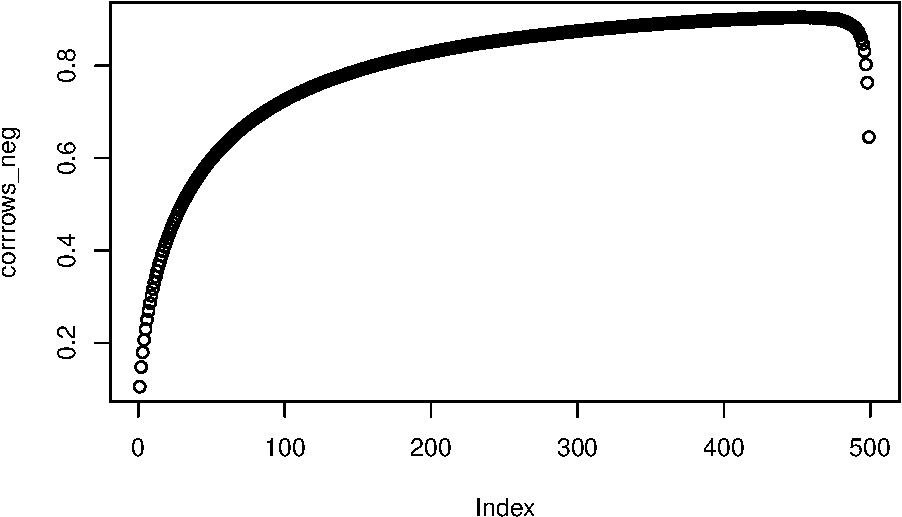
\includegraphics{Exercise_1_files/figure-latex/unnamed-chunk-22-1.pdf}

\begin{itemize}
\tightlist
\item
  quite resembles a gaussian distribution with mean between 50-70
\item
  light leftmost bin frequency
\end{itemize}

\hypertarget{boxplots}{%
\subsubsection{Boxplots}\label{boxplots}}

\begin{Shaded}
\begin{Highlighting}[]
\CommentTok{# setting plot sizes}
\KeywordTok{options}\NormalTok{(}\DataTypeTok{repr.plot.width =} \DecValTok{18}\NormalTok{, }\DataTypeTok{repr.plot.height =} \DecValTok{10}\NormalTok{)}
\end{Highlighting}
\end{Shaded}

\begin{Shaded}
\begin{Highlighting}[]
\CommentTok{# numeric columns}
\NormalTok{cols =}\StringTok{ }\KeywordTok{colnames}\NormalTok{(d)[}\KeywordTok{colnames}\NormalTok{(d) }\OperatorTok{!=}\StringTok{ 'X'} \OperatorTok{&}\StringTok{ }\KeywordTok{colnames}\NormalTok{(d) }\OperatorTok{!=}\StringTok{ 'Private'}\NormalTok{]}

\CommentTok{# maximum per column}
\KeywordTok{sapply}\NormalTok{(d }\OperatorTok\StringTok{ }\NormalTok{dplyr}\OperatorTok{::}\KeywordTok{select}\NormalTok{(cols), max, }\DataTypeTok{na.rm =} \OtherTok{TRUE}\NormalTok{)}
\end{Highlighting}
\end{Shaded}

\begin{verbatim}
## Note: Using an external vector in selections is ambiguous.
## i Use `all_of(cols)` instead of `cols` to silence this message.
## i See <https://tidyselect.r-lib.org/reference/faq-external-vector.html>.
## This message is displayed once per session.
\end{verbatim}

\begin{verbatim}
##        Apps      Accept      Enroll   Top10perc   Top25perc F.Undergrad 
##     48094.0     26330.0      6392.0        96.0       100.0     31643.0 
## P.Undergrad    Outstate  Room.Board       Books    Personal         PhD 
##     21836.0     21700.0      8124.0      2340.0      6800.0       103.0 
##    Terminal   S.F.Ratio perc.alumni      Expend   Grad.Rate 
##       100.0        39.8        64.0     56233.0       118.0
\end{verbatim}

\begin{Shaded}
\begin{Highlighting}[]
\CommentTok{# low val cols}
\NormalTok{low_val_c =}\StringTok{ }\KeywordTok{c}\NormalTok{(}\StringTok{'Top10perc'}\NormalTok{,}\StringTok{'Top25perc'}\NormalTok{,}\StringTok{'PhD'}\NormalTok{,}\StringTok{'Terminal'}\NormalTok{,}\StringTok{'S.F.Ratio'}\NormalTok{,}\StringTok{'perc.alumni'}\NormalTok{,}\StringTok{'Grad.Rate'}\NormalTok{)}
\NormalTok{low_val =}\StringTok{ }\KeywordTok{melt}\NormalTok{(d, }\DataTypeTok{id.vars=}\StringTok{'X'}\NormalTok{, }\DataTypeTok{measure.vars=}\NormalTok{low_val_c)}

\CommentTok{# med val cols}
\NormalTok{med_val_c =}\StringTok{ }\KeywordTok{c}\NormalTok{(}\StringTok{'Enroll'}\NormalTok{,}\StringTok{'Room.Board'}\NormalTok{,}\StringTok{'Books'}\NormalTok{,}\StringTok{'Personal'}\NormalTok{)}
\NormalTok{med_val =}\StringTok{ }\KeywordTok{melt}\NormalTok{(d, }\DataTypeTok{id.vars=}\StringTok{'X'}\NormalTok{, }\DataTypeTok{measure.vars=}\NormalTok{med_val_c)}

\CommentTok{# high val cols}
\NormalTok{high_val_c =}\StringTok{ }\KeywordTok{c}\NormalTok{(}\StringTok{'Apps'}\NormalTok{,}\StringTok{'Accept'}\NormalTok{,}\StringTok{'F.Undergrad'}\NormalTok{,}\StringTok{'P.Undergrad'}\NormalTok{,}\StringTok{'Outstate'}\NormalTok{,}\StringTok{'Expend'}\NormalTok{)}
\NormalTok{high_val =}\StringTok{ }\KeywordTok{melt}\NormalTok{(d, }\DataTypeTok{id.vars=}\StringTok{'X'}\NormalTok{, }\DataTypeTok{measure.vars=}\NormalTok{high_val_c)}
\end{Highlighting}
\end{Shaded}

\hypertarget{variables-with-low-values-maximum-under-120}{%
\paragraph{Variables with low values (maximum under
120)}\label{variables-with-low-values-maximum-under-120}}

\begin{Shaded}
\begin{Highlighting}[]
\NormalTok{low_val }\OperatorTok
\StringTok{    }\KeywordTok{ggplot}\NormalTok{(}\KeywordTok{aes}\NormalTok{(}\DataTypeTok{x=}\StringTok{"X"}\NormalTok{, }\DataTypeTok{y=}\NormalTok{value)) }\OperatorTok{+}
\StringTok{    }\KeywordTok{geom_boxplot}\NormalTok{(}\KeywordTok{aes}\NormalTok{(}\DataTypeTok{color=}\NormalTok{variable))}
\end{Highlighting}
\end{Shaded}

\includegraphics{Exercise_1_files/figure-latex/unnamed-chunk-25-1.pdf}

\begin{Shaded}
\begin{Highlighting}[]
\CommentTok{# quantiles}
\KeywordTok{sapply}\NormalTok{(d }\OperatorTok\StringTok{ }\NormalTok{dplyr}\OperatorTok{::}\KeywordTok{select}\NormalTok{(low_val_c), quantile, }\DataTypeTok{na.rm =} \OtherTok{TRUE}\NormalTok{)}
\end{Highlighting}
\end{Shaded}

\begin{verbatim}
## Note: Using an external vector in selections is ambiguous.
## i Use `all_of(low_val_c)` instead of `low_val_c` to silence this message.
## i See <https://tidyselect.r-lib.org/reference/faq-external-vector.html>.
## This message is displayed once per session.
\end{verbatim}

\begin{verbatim}
##      Top10perc Top25perc PhD Terminal S.F.Ratio perc.alumni Grad.Rate
## 0%           1         9   8       24       2.5           0        10
## 25%         15        41  62       71      11.5          13        53
## 50%         23        54  75       82      13.6          21        65
## 75%         35        69  85       92      16.5          31        78
## 100%        96       100 103      100      39.8          64       118
\end{verbatim}

For the low value variables we can notice a few things:

\begin{itemize}
\tightlist
\item
  Top10perc
\end{itemize}

In our boxplot we can see that the median for this variable is 23, the
maximum is 96 and the minimum is 1 with the 25\% and 75\% percentiles
sitting at 15 and 35 respectively.

The range for this variable is of 95 and the IQR (interquartile range)
is equal to 20.

\begin{itemize}
\tightlist
\item
  Top25perc
\end{itemize}

In our boxplot we can see that the median for this variable is 54, the
maximum is 100 and the minimum is 9 with the 25\% and 75\% percentiles
sitting at 41 and 69 respectively.

The range for this variable is of 91 and the IQR is equal to 28

\begin{itemize}
\tightlist
\item
  PhD
\end{itemize}

In our boxplot we can see that the median for this variable is 75, the
maximum is 103 and the minimum is 8 with the 25\% and 75\% percentiles
sitting at 62 and 85 respectively.

The range for this variable is of 95 and the IQR is equal to 23

\begin{itemize}
\tightlist
\item
  Terminal
\end{itemize}

In our boxplot we can see that the median for this variable is 82, the
maximum is 100 and the minimum is 24 with the 25\% and 75\% percentiles
sitting at 71 and 92 respectively.

The range for this variable is of 76 and the IQR is equal to 21

\begin{itemize}
\tightlist
\item
  S.F.Ratio
\end{itemize}

In our boxplot we can see that the median for this variable is 13.6, the
maximum is 39.8 and the minimum is 2.5 with the 25\% and 75\%
percentiles sitting at 11.5 and 16.5 respectively.

The range for this variable is of 37.3 and the IQR is equal to 5

\begin{itemize}
\tightlist
\item
  perc.alumni
\end{itemize}

In our boxplot we can see that the median for this variable is 21, the
maximum is 64 and the minimum is 0 with the 25\% and 75\% percentiles
sitting at 13 and 31 respectively.

The range for this variable is of 64 and the IQR is equal to 18

\begin{itemize}
\tightlist
\item
  Grad.Rate
\end{itemize}

In our boxplot we can see that the median for this variable is 65, the
maximum is 118 and the minimum is 10 with the 25\% and 75\% percentiles
sitting at 53 and 78 respectively.

The range for this variable is of 108 and the IQR is equal to 25

\hypertarget{variables-with-medium-values-maximum-less-than-or-equal-to-8124-and-not-in-low-values-list}{%
\paragraph{Variables with medium values (maximum less than or equal to
8124 and not in low values
list)}\label{variables-with-medium-values-maximum-less-than-or-equal-to-8124-and-not-in-low-values-list}}

\begin{Shaded}
\begin{Highlighting}[]
\NormalTok{med_val }\OperatorTok
\StringTok{    }\KeywordTok{ggplot}\NormalTok{(}\KeywordTok{aes}\NormalTok{(}\DataTypeTok{x=}\StringTok{"X"}\NormalTok{, }\DataTypeTok{y=}\NormalTok{value)) }\OperatorTok{+}
\StringTok{    }\KeywordTok{geom_boxplot}\NormalTok{(}\KeywordTok{aes}\NormalTok{(}\DataTypeTok{color=}\NormalTok{variable))}
\end{Highlighting}
\end{Shaded}

\includegraphics{Exercise_1_files/figure-latex/unnamed-chunk-27-1.pdf}

\begin{Shaded}
\begin{Highlighting}[]
\CommentTok{# quantiles}
\KeywordTok{sapply}\NormalTok{(d }\OperatorTok\StringTok{ }\NormalTok{dplyr}\OperatorTok{::}\KeywordTok{select}\NormalTok{(med_val_c), quantile, }\DataTypeTok{na.rm =} \OtherTok{TRUE}\NormalTok{)}
\end{Highlighting}
\end{Shaded}

\begin{verbatim}
## Note: Using an external vector in selections is ambiguous.
## i Use `all_of(med_val_c)` instead of `med_val_c` to silence this message.
## i See <https://tidyselect.r-lib.org/reference/faq-external-vector.html>.
## This message is displayed once per session.
\end{verbatim}

\begin{verbatim}
##      Enroll Room.Board Books Personal
## 0%       35       1780    96      250
## 25%     242       3597   470      850
## 50%     434       4200   500     1200
## 75%     902       5050   600     1700
## 100%   6392       8124  2340     6800
\end{verbatim}

For the medium value variables we can notice a few things:

\begin{itemize}
\tightlist
\item
  Enroll
\end{itemize}

In our boxplot we can see that the median for this variable is 494, the
maximum is 6392 and the minimum is 35 with the 25\% and 75\% percentiles
sitting at 242 and 902 respectively.

The range for this variable is of 6357 and the IQR (interquartile range)
is equal to 660.

\begin{itemize}
\tightlist
\item
  Room.Board
\end{itemize}

In our boxplot we can see that the median for this variable is 4200, the
maximum is 8124 and the minimum is 1780 with the 25\% and 75\%
percentiles sitting at 3597 and 5050 respectively.

The range for this variable is of 6344 and the IQR is equal to 1453.

\begin{itemize}
\tightlist
\item
  Books
\end{itemize}

In our boxplot we can see that the median for this variable is 500, the
maximum is 2340 and the minimum is 96 with the 25\% and 75\% percentiles
sitting at 470 and 600 respectively.

The range for this variable is of 2244 and the IQR is equal to 130

\begin{itemize}
\tightlist
\item
  Personal
\end{itemize}

In our boxplot we can see that the median for this variable is 1200, the
maximum is 6800 and the minimum is 250 with the 25\% and 75\%
percentiles sitting at 850 and 1700 respectively.

The range for this variable is of 6550 and the IQR is equal to 850

\hypertarget{variables-with-high-values-maximums-above-8124}{%
\paragraph{Variables with high values (maximums above
8124)}\label{variables-with-high-values-maximums-above-8124}}

\begin{Shaded}
\begin{Highlighting}[]
\NormalTok{high_val }\OperatorTok
\StringTok{    }\KeywordTok{ggplot}\NormalTok{(}\KeywordTok{aes}\NormalTok{(}\DataTypeTok{x=}\StringTok{"X"}\NormalTok{, }\DataTypeTok{y=}\NormalTok{value)) }\OperatorTok{+}
\StringTok{    }\KeywordTok{geom_boxplot}\NormalTok{(}\KeywordTok{aes}\NormalTok{(}\DataTypeTok{color=}\NormalTok{variable))}
\end{Highlighting}
\end{Shaded}

\includegraphics{Exercise_1_files/figure-latex/unnamed-chunk-29-1.pdf}

\begin{Shaded}
\begin{Highlighting}[]
\CommentTok{# quantiles}
\KeywordTok{sapply}\NormalTok{(d }\OperatorTok\StringTok{ }\NormalTok{dplyr}\OperatorTok{::}\KeywordTok{select}\NormalTok{(high_val_c), quantile, }\DataTypeTok{na.rm =} \OtherTok{TRUE}\NormalTok{)}
\end{Highlighting}
\end{Shaded}

\begin{verbatim}
## Note: Using an external vector in selections is ambiguous.
## i Use `all_of(high_val_c)` instead of `high_val_c` to silence this message.
## i See <https://tidyselect.r-lib.org/reference/faq-external-vector.html>.
## This message is displayed once per session.
\end{verbatim}

\begin{verbatim}
##       Apps Accept F.Undergrad P.Undergrad Outstate Expend
## 0%      81     72         139           1     2340   3186
## 25%    776    604         992          95     7320   6751
## 50%   1558   1110        1707         353     9990   8377
## 75%   3624   2424        4005         967    12925  10830
## 100% 48094  26330       31643       21836    21700  56233
\end{verbatim}

For the high value variables we can notice a few things:

\begin{itemize}
\tightlist
\item
  Apps
\end{itemize}

In our boxplot we can see that the median for this variable is 1558, the
maximum is 48094 and the minimum is 81 with the 25\% and 75\%
percentiles sitting at 776 and 3624 respectively.

The range for this variable is of 48013 and the IQR (interquartile
range) is equal to 2848.

\begin{itemize}
\tightlist
\item
  Accept
\end{itemize}

In our boxplot we can see that the median for this variable is 1110, the
maximum is 26330 and the minimum is 72 with the 25\% and 75\%
percentiles sitting at 604 and 2424 respectively.

The range for this variable is of 26258 and the IQR is equal to 1820.

\begin{itemize}
\tightlist
\item
  F.Undergrad
\end{itemize}

In our boxplot we can see that the median for this variable is 1707, the
maximum is 31643 and the minimum is 139 with the 25\% and 75\%
percentiles sitting at 992 and 4005 respectively.

The range for this variable is of 31504 and the IQR is equal to 3013

\begin{itemize}
\tightlist
\item
  P.Undergrad
\end{itemize}

In our boxplot we can see that the median for this variable is 353, the
maximum is 21836 and the minimum is 1 with the 25\% and 75\% percentiles
sitting at 95 and 967 respectively.

The range for this variable is of 21835 and the IQR is equal to 872

\begin{itemize}
\tightlist
\item
  Outstate
\end{itemize}

In our boxplot we can see that the median for this variable is 9990, the
maximum is 21700 and the minimum is 2340 with the 25\% and 75\%
percentiles sitting at 7320 and 12925 respectively.

The range for this variable is of 19360 and the IQR is equal to 5605

\begin{itemize}
\tightlist
\item
  Expend
\end{itemize}

In our boxplot we can see that the median for this variable is 8377, the
maximum is 56233 and the minimum is 3186 with the 25\% and 75\%
percentiles sitting at 6751 and 10830 respectively.

The range for this variable is of 53047 and the IQR is equal to 4079

\hypertarget{perform-a-visual-analysis-of-all-quantitative-variables-together.-then-perform-a-visual-analysis-of-each-of-the-quantitative-variables-taking-into-account-the-variable-private.}{%
\subsection{3- Perform a visual analysis of all quantitative variables
together. Then, Perform a visual analysis of each of the quantitative
variables taking into account the variable
Private.}\label{perform-a-visual-analysis-of-all-quantitative-variables-together.-then-perform-a-visual-analysis-of-each-of-the-quantitative-variables-taking-into-account-the-variable-private.}}

\hypertarget{correlation-and-scatterplots-for-all-variables}{%
\subsubsection{Correlation and scatterplots for all
variables}\label{correlation-and-scatterplots-for-all-variables}}

\begin{Shaded}
\begin{Highlighting}[]
\NormalTok{pa <-}\StringTok{ }\NormalTok{d }\OperatorTok\StringTok{ }\NormalTok{dplyr}\OperatorTok{::}\KeywordTok{select}\NormalTok{(cols)}
\KeywordTok{chart.Correlation}\NormalTok{(pa, }\DataTypeTok{histogram=}\OtherTok{TRUE}\NormalTok{, }\DataTypeTok{pch=}\DecValTok{19}\NormalTok{, }\DataTypeTok{method=}\StringTok{"pearson"}\NormalTok{)}
\end{Highlighting}
\end{Shaded}

\includegraphics{Exercise_1_files/figure-latex/unnamed-chunk-31-1.pdf}

Here we can see a plot with all the numerical variables, a histogram and
density plot in the main diagonal. To the bottom of the diagonal we see
scatterplots for each pair of variables and a line that goes through the
scatterplot. Above the main diagonal we see all the correlation
coefficients for each pair of variables.

We see there are some highly correlated variables and some others which
have negligible correlation.

All correlation coefficients are Pearson correlation coefficients.

The variables with the highest correlation are the following:

\begin{itemize}
\tightlist
\item
  F.Undergrad vs Enroll with very high correlation of 0.96
\item
  Apps vs Accept with a similarly high correlation coefficient of 0.94
\item
  Accept vs Enroll also have a very high correlation of 0.91
\item
  Top10perc vs Top25perc have a correlation of 0.89
\item
  F.Undergrad vs Accept have a correlation of 0.
\item
  Both Apps vs Enroll and Phd vs Terminal have a correlation of 0.85
\end{itemize}

\begin{Shaded}
\begin{Highlighting}[]
\CommentTok{# setting colors}
\NormalTok{color_}\DecValTok{1}\NormalTok{ <-}\StringTok{ "black"}
\NormalTok{color_}\DecValTok{2}\NormalTok{ <-}\StringTok{ "red"}
\NormalTok{colors <-}\StringTok{ }\KeywordTok{as.numeric}\NormalTok{(}\KeywordTok{as.factor}\NormalTok{(d}\OperatorTok{$}\NormalTok{Private)) }\OperatorTok{-}\StringTok{ }\DecValTok{1}
\NormalTok{i <-}\StringTok{ }\DecValTok{1}
\ControlFlowTok{for}\NormalTok{ (num }\ControlFlowTok{in}\NormalTok{ colors) \{}
\NormalTok{    colors[i] =}\StringTok{ }\KeywordTok{ifelse}\NormalTok{(num}\OperatorTok{==}\DecValTok{1}\NormalTok{, color_}\DecValTok{1}\NormalTok{, color_}\DecValTok{2}\NormalTok{)}
\NormalTok{    i <-}\StringTok{ }\NormalTok{i }\OperatorTok{+}\StringTok{ }\DecValTok{1}
\NormalTok{\}}
\end{Highlighting}
\end{Shaded}

\begin{Shaded}
\begin{Highlighting}[]
\NormalTok{pa <-}\StringTok{ }\NormalTok{d }\OperatorTok\StringTok{ }\NormalTok{dplyr}\OperatorTok{::}\KeywordTok{select}\NormalTok{(cols)}
\KeywordTok{pairs}\NormalTok{(pa,}\DataTypeTok{pch=}\DecValTok{1}\NormalTok{,}\DataTypeTok{col=}\NormalTok{colors)}
\end{Highlighting}
\end{Shaded}

\includegraphics{Exercise_1_files/figure-latex/unnamed-chunk-33-1.pdf}

In most of these scatter plots we see an interesting pattern, where for
varibles plotted versus Top10perc, Top20perc, PhD and Terminal there
seems to be no clear divide between each one ofg the groups, except when
compared to variables that significantly diffentiate both groups.

The clear differentiator variables seem to be P.Undergrad, F.Undergrad,
S.F.Ratio, Apps, Accept, Enrool and outstate.

And sure, I could definitely agree that the size of each plot might be
overestimating such division in groups, but some of these variables do
show a stark difference in values.

\hypertarget{pcp}{%
\subsubsection{PCP}\label{pcp}}

\begin{Shaded}
\begin{Highlighting}[]
\KeywordTok{parcoord}\NormalTok{(pa,}\DataTypeTok{var.label=}\OtherTok{TRUE}\NormalTok{)}
\end{Highlighting}
\end{Shaded}

\includegraphics{Exercise_1_files/figure-latex/unnamed-chunk-34-1.pdf}

We can basically just see the spread of the data here, the only thing I
take from it is that apps and accept have really very few outliers in
terms of quantity, but they're significantly larger than the rest. Shows
how skewed these variables are.

\begin{Shaded}
\begin{Highlighting}[]
\KeywordTok{parcoord}\NormalTok{(pa,}\DataTypeTok{var.label=}\OtherTok{TRUE}\NormalTok{, }\DataTypeTok{col=}\NormalTok{colors)}
\end{Highlighting}
\end{Shaded}

\includegraphics{Exercise_1_files/figure-latex/unnamed-chunk-35-1.pdf}

We can see that the more extreme variables of Apps, Accept, P.Undergrad,
F.Undergrad seem to be affected by whether it's private or not.

In the case of outstate too, but instead of being the highest values,
the values where it's private correspond to the lowest values.

For Grad.Rate it also seem somewhat divided and in a similar way for
perc.alumni.

For Top10perc, Top25perc, PhD or Terminal there seems to be no
noticeable difference made by whether it's private or not.

\hypertarget{randomizing-the-order-of-the-variables-we-get-a-different-but-perhaps-better-pcp.}{%
\paragraph{Randomizing the order of the variables we get a different but
perhaps better
PCP.}\label{randomizing-the-order-of-the-variables-we-get-a-different-but-perhaps-better-pcp.}}

\begin{Shaded}
\begin{Highlighting}[]
\NormalTok{cols <-}\StringTok{ }\KeywordTok{sample}\NormalTok{(cols)}
\NormalTok{pa <-}\StringTok{ }\NormalTok{pa }\OperatorTok\StringTok{ }\NormalTok{dplyr}\OperatorTok{::}\KeywordTok{select}\NormalTok{(cols)}
\KeywordTok{parcoord}\NormalTok{(pa,}\DataTypeTok{var.label=}\OtherTok{TRUE}\NormalTok{, }\DataTypeTok{col=}\NormalTok{colors)}
\end{Highlighting}
\end{Shaded}

\includegraphics{Exercise_1_files/figure-latex/unnamed-chunk-36-1.pdf}

Here we can more clearly see that for S.F.Ratio there is a stark
difference between both groups, where the group labeled as Private seems
to have the higher values.

For the rest of the variables we get much of the same we explained
earlier.

\hypertarget{if-we-were-to-line-up-variables-with-similarly-shaped-histograms-we-could-get-an-interesting-pcp-lets-try-that.}{%
\paragraph{If we were to line up variables with similarly shaped
histograms, we could get an interesting PCP, let's try
that.}\label{if-we-were-to-line-up-variables-with-similarly-shaped-histograms-we-could-get-an-interesting-pcp-lets-try-that.}}

We will exclude Top10perc and Top25perc as these do not contribute too
much to the plot

\begin{Shaded}
\begin{Highlighting}[]
\CommentTok{# right skewed variables}
\NormalTok{right_skewed <-}\StringTok{ }\KeywordTok{c}\NormalTok{(}\StringTok{'Apps'}\NormalTok{,}\StringTok{'Accept'}\NormalTok{,}\StringTok{'P.Undergrad'}\NormalTok{,}\StringTok{'F.Undergrad'}\NormalTok{,}\StringTok{'Personal'}\NormalTok{,}\StringTok{'Expend'}\NormalTok{,}\StringTok{'Books'}\NormalTok{,}\StringTok{'perc.alumni'}\NormalTok{)}
\NormalTok{right_skewed <-}\StringTok{ }\NormalTok{d }\OperatorTok\StringTok{ }\NormalTok{dplyr}\OperatorTok{::}\KeywordTok{select}\NormalTok{(right_skewed)}
\end{Highlighting}
\end{Shaded}

\begin{verbatim}
## Note: Using an external vector in selections is ambiguous.
## i Use `all_of(right_skewed)` instead of `right_skewed` to silence this message.
## i See <https://tidyselect.r-lib.org/reference/faq-external-vector.html>.
## This message is displayed once per session.
\end{verbatim}

\begin{Shaded}
\begin{Highlighting}[]
\CommentTok{# normal-like variables}
\NormalTok{normal_like <-}\StringTok{ }\KeywordTok{c}\NormalTok{(}\StringTok{'Outstate'}\NormalTok{,}\StringTok{'Room.Board'}\NormalTok{,}\StringTok{'perc.alumni'}\NormalTok{,}\StringTok{'Grad.Rate'}\NormalTok{,}\StringTok{'S.F.Ratio'}\NormalTok{)}
\NormalTok{normal_like <-}\StringTok{ }\NormalTok{d }\OperatorTok\StringTok{ }\NormalTok{dplyr}\OperatorTok{::}\KeywordTok{select}\NormalTok{(normal_like)}
\end{Highlighting}
\end{Shaded}

\begin{verbatim}
## Note: Using an external vector in selections is ambiguous.
## i Use `all_of(normal_like)` instead of `normal_like` to silence this message.
## i See <https://tidyselect.r-lib.org/reference/faq-external-vector.html>.
## This message is displayed once per session.
\end{verbatim}

\begin{Shaded}
\begin{Highlighting}[]
\CommentTok{# left skewed variables}
\NormalTok{left_skewed <-}\StringTok{ }\KeywordTok{c}\NormalTok{(}\StringTok{'PhD'}\NormalTok{,}\StringTok{'Terminal'}\NormalTok{)}
\NormalTok{left_skewed <-}\StringTok{ }\NormalTok{d }\OperatorTok\StringTok{ }\NormalTok{dplyr}\OperatorTok{::}\KeywordTok{select}\NormalTok{(left_skewed)}
\end{Highlighting}
\end{Shaded}

\begin{verbatim}
## Note: Using an external vector in selections is ambiguous.
## i Use `all_of(left_skewed)` instead of `left_skewed` to silence this message.
## i See <https://tidyselect.r-lib.org/reference/faq-external-vector.html>.
## This message is displayed once per session.
\end{verbatim}

\hypertarget{right-skewed-variables-pcp}{%
\paragraph{right skewed variables
PCP}\label{right-skewed-variables-pcp}}

\begin{Shaded}
\begin{Highlighting}[]
\KeywordTok{parcoord}\NormalTok{(right_skewed,}\DataTypeTok{var.label=}\OtherTok{TRUE}\NormalTok{, }\DataTypeTok{col=}\NormalTok{colors)}
\end{Highlighting}
\end{Shaded}

\includegraphics{Exercise_1_files/figure-latex/unnamed-chunk-38-1.pdf}

After grouping similarly shaped variables the plots are somewhat
clearer. Confirming most of our previous observations.

The general idea is that for these variables, pretty much everything but
perc.alumni, Books and Expend follow a pattern where the
higher-than-usual variables pretty much belong completely to entries of
Private colleges.

\hypertarget{normal-like-variables-pcp}{%
\paragraph{normal-like variables PCP}\label{normal-like-variables-pcp}}

\begin{Shaded}
\begin{Highlighting}[]
\KeywordTok{parcoord}\NormalTok{(normal_like,}\DataTypeTok{var.label=}\OtherTok{TRUE}\NormalTok{, }\DataTypeTok{col=}\NormalTok{colors)}
\end{Highlighting}
\end{Shaded}

\includegraphics{Exercise_1_files/figure-latex/unnamed-chunk-39-1.pdf}

I particularly like this one. These variables look significantly clearer
here than in the first PCP.

The first observations still hold though. For pretty much all these
variables there's a significant divide in the same direction except for
S.F.Ratio where that pattern is inverted.

\hypertarget{left-skewed-variables-pcp}{%
\paragraph{left skewed variables PCP}\label{left-skewed-variables-pcp}}

\begin{Shaded}
\begin{Highlighting}[]
\KeywordTok{parcoord}\NormalTok{(left_skewed,}\DataTypeTok{var.label=}\OtherTok{TRUE}\NormalTok{, }\DataTypeTok{col=}\NormalTok{colors)}
\end{Highlighting}
\end{Shaded}

\includegraphics{Exercise_1_files/figure-latex/unnamed-chunk-40-1.pdf}

being private or not makes no difference here, therefore not very
interesting.

\hypertarget{andrews-plot}{%
\subsubsection{Andrews' plot}\label{andrews-plot}}

\begin{Shaded}
\begin{Highlighting}[]
\KeywordTok{par}\NormalTok{(}\DataTypeTok{mfrow=}\KeywordTok{c}\NormalTok{(}\DecValTok{1}\NormalTok{,}\DecValTok{1}\NormalTok{))}
\KeywordTok{andrews}\NormalTok{(}\KeywordTok{as.data.frame}\NormalTok{(}\KeywordTok{cbind}\NormalTok{(pa,}\KeywordTok{as.factor}\NormalTok{(d}\OperatorTok{$}\NormalTok{Private))),}\DataTypeTok{clr=}\DecValTok{7}\NormalTok{,}\DataTypeTok{ymax=}\DecValTok{6}\NormalTok{)}
\end{Highlighting}
\end{Shaded}

\includegraphics{Exercise_1_files/figure-latex/unnamed-chunk-41-1.pdf}

The Andrews' plot makes it difficult to appreciate a significant
difference between both groups in my opinion. Perhaps I might need to
read up more on it but it doesn't show tell me too much about the values
other than around the middle. Where the we have the 0 and around -2,
where the groups seem more divided than everywhere else, taking
different directions in the dataset.

\end{document}
